\documentclass{article}
\usepackage{tikz}

\begin{document}

% Original network
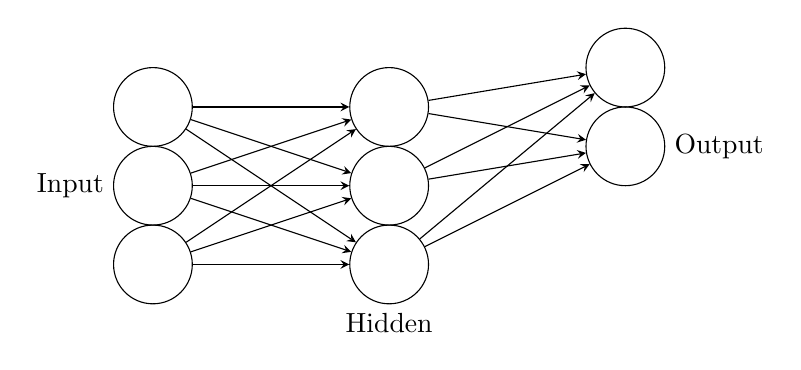
\begin{tikzpicture}[
    layer/.style={circle, draw, minimum size=1cm},
    >=stealth
]
% Input layer
\foreach \i in {1,2,3} {
    \node[layer] (I\i) at (0,\i) {};
}

% Hidden layer
\foreach \i in {1,2,3} {
    \node[layer] (H\i) at (3,\i) {};
}

% Output layer
\foreach \i in {1,2} {
    \node[layer] (O\i) at (6,1.5+\i) {};
}

% Connections
\foreach \i in {1,2,3} {
    \foreach \j in {1,2,3} {
        \draw[->] (I\i) -- (H\j);
    }
}

\foreach \i in {1,2,3} {
    \foreach \j in {1,2} {
        \draw[->] (H\i) -- (O\j);
    }
}

% Labels
\node[left] at (-0.5,2) {Input};
\node[below] at (3,0.5) {Hidden};
\node[right] at (6.5,2.5) {Output};
\end{tikzpicture}

% Add some vertical space
\vspace{2cm}

% Larger network with extra hidden layer
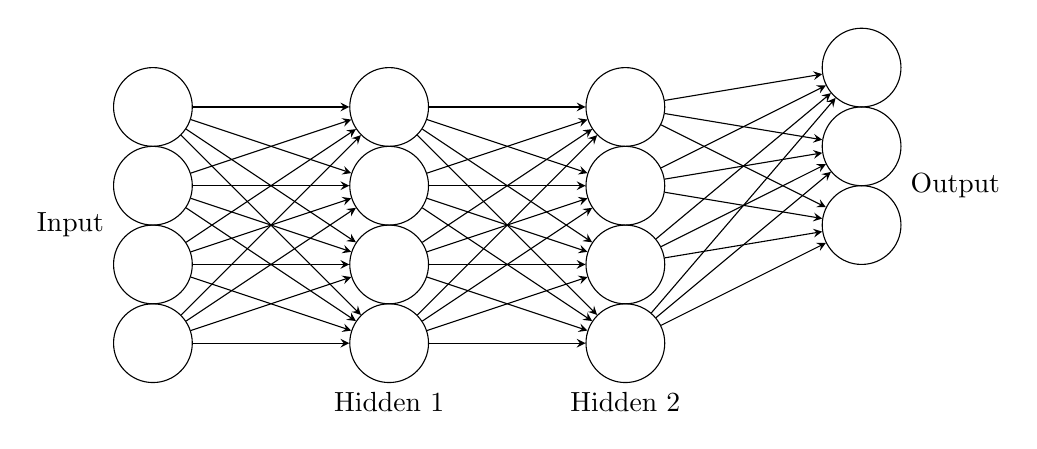
\begin{tikzpicture}[
    layer/.style={circle, draw, minimum size=1cm},
    >=stealth
]
% Input layer
\foreach \i in {1,2,3,4} {
    \node[layer] (I\i) at (0,\i) {};
}

% First Hidden layer
\foreach \i in {1,2,3,4} {
    \node[layer] (H1\i) at (3,\i) {};
}

% Second Hidden layer
\foreach \i in {1,2,3,4} {
    \node[layer] (H2\i) at (6,\i) {};
}

% Output layer
\foreach \i in {1,2,3} {
    \node[layer] (O\i) at (9,1.5+\i) {};
}

% Connections
\foreach \i in {1,2,3,4} {
    \foreach \j in {1,2,3,4} {
        \draw[->] (I\i) -- (H1\j);
    }
}

\foreach \i in {1,2,3,4} {
    \foreach \j in {1,2,3,4} {
        \draw[->] (H1\i) -- (H2\j);
    }
}

\foreach \i in {1,2,3,4} {
    \foreach \j in {1,2,3} {
        \draw[->] (H2\i) -- (O\j);
    }
}

% Labels
\node[left] at (-0.5,2.5) {Input};
\node[below] at (3,0.5) {Hidden 1};
\node[below] at (6,0.5) {Hidden 2};
\node[right] at (9.5,3) {Output};
\end{tikzpicture}

\end{document} 
